%
% File ling_581_F2024.tex
%
% Contact: dkdougal@byu.edu
%%
%% Based on the style files for ACL-2015 & ACL-2019

\documentclass[11pt,table,xcdraw]{article}
\usepackage[hyperref]{tex_styles/acl2019_no_nums}

\usepackage{import}
\import{./}{tex_styles/preamble.tex}

\graphicspath{{images/}}

\setlength\titlebox{5 cm}

% Turn off hyphenation 
%\hyphenpenalty=10000 
%\exhyphenpenalty=10000

%\newcommand\BibTeX{B\textsc{ib}\TeX}

\title{Instructions for LING 581 Research Paper}

\author{Your Name \\
  Linguistics 581, Section 002, Winter 2025 \\
  Submitted to Professor Dougal \\
  Department of Linguistics \\
  Brigham Young University \\
  {\tt your.email@byu.edu} }

\date{}

\begin{document}

\maketitle

\begin{abstract}
This document contains the instructions for preparing a submission-ready manuscript for your research project for LING 581. The document itself conforms to its own specifications, and is therefore an example of what your manuscript should look like. These instructions should be used for final versions of submitted papers. You must conform to all the directions reported in this document. [For your final paper submission, you may use an AI-generated summary of your full report \textit{for the Abstract section only} so long as you cite the proper AI attribution like this~\cite{chatgpt}.]
\end{abstract}


\section{Introduction}

This document serves as a template with examples for your final paper. Become familiar with the examples and the use of \LaTeX\ source code.

\section{Credits}

This document has been adapted from the instructions for Association for Computational Linguistics (ACL) proceedings, primarily those for ACL-2015 and ACL-2019. Additional elements were taken from the formatting instructions of the {\em International Joint Conference on Artificial Intelligence} and of the {\em International Conference on Language Resources and Evaluation}.

\section{Instructions}

The following instructions are directed to authors of papers submitted to LING 581. All authors are required to adhere to these specifications. Authors are required to provide a Portable Document Format (PDF) version of their papers. \textbf{The proceedings are designed for printing on A4 paper.}


\subsection{General Instructions} 

\begin{enumerate}
    \item Manuscripts must be in two-column format as facilitated by this template and stylesheet.  Exceptions to the two-column format include the title block with title, author's name, and complete submission address (class, section, semester, professor, department, and university), which must be centered at the top of the first page, and any full-width figures or tables (see the guidelines in Subsection~\ref{ssec:first}). 
    \item {\bf Type single-spaced.}  
    \item Start all pages directly under the top margin as provided by the template. See the guidelines later regarding formatting the first page.  
    \item The manuscript should be printed single-sided and its length should not exceed the maximum page limit described in Section~\ref{sec:length}. 
    \item For professional journal submissions, pages are not numbered; however, pages are numbered for this assignment use.
\end{enumerate}


\subsection{Electronically-available resources}

For the production of the electronic manuscript you must use Adobe's Portable Document Format (PDF). To receive credit for submitting your final paper and other assignments throughout the class, you must prepare your PDF files using \LaTeX\ with the slightly modified ACL 2019 content style and bibliography style files:

\begin{itemize}
    \item \texttt{acl2019.sty}
    \item \texttt{acl2019\_no\_nums.sty}
    \item \texttt{acl\_natbib.bst} 
    \item \texttt{acl\_natbib\_no\_note.bst}
\end{itemize}


You will find the document you are currently reading and its \LaTeX\ source code and other resources on the class LMS:

\begin{itemize}
    \item \texttt{ling\_581\_Instructions.pdf}
    \item \texttt{ling\_581\_Instructions.tex}
\end{itemize}

Using \href{http://www.overleaf.com}{Overleaf} is the preferred and recommended tool for creating your \LaTeX\ documents.


\subsection{Format of Electronic Manuscript}
\label{sect:pdf}

Please make sure that your PDF file includes all the necessary fonts (especially tree diagrams, symbols, and fonts with Asian characters). When you print or create the PDF file, there is usually
an option in your printer setup to include none, all or just non-standard fonts.  Please make sure that you select the option of including ALL the fonts. Print-outs of the PDF file on A4 paper should be identical to the hardcopy version. 


\subsection{Fonts}

For reasons of uniformity, Adobe's {\bf Times Roman} font should be used as facilitated by this template and stylesheet. In \LaTeX2e{} this is accomplished by putting

\begin{quote}
\begin{verbatim}
\usepackage{times}
\usepackage{latexsym}
\end{verbatim}
\end{quote}
in the preamble. If Times Roman is unavailable, use {\bf Computer
  Modern Roman} (\LaTeX2e{}'s default).  Note that the latter is about
  10\% less dense than Adobe's Times Roman font.


\begin{table}[h]
\begin{center}
\begin{tabular}{|l|r|l|}
\hline \bf Type of Text & \bf Font Size & \bf Style \\ \hline
paper title & 15 pt & bold \\
author names & 12 pt & bold \\
author affiliation & 12 pt & \\
the word ``Abstract'' & 12 pt & bold \\
section titles & 12 pt & bold \\
document text & 11 pt  &\\
captions & 11 pt & \\
abstract text & 10 pt & \\
bibliography & 10 pt & \\
footnotes & 9 pt & \\
\hline
\end{tabular}
\end{center}
\caption{\label{font-table} Font guide. }
\end{table}

\subsection{The First Page}
\label{ssec:first}

Center the title, author's name(s) and affiliation(s) across both columns. Do not use footnotes for affiliations. Use the two-column format only when you begin the abstract.

\begin{itemize}
\item {\bf Title}: Place the title centered at the top of the first page, in
a 15-point bold font. (For a complete guide to font sizes and styles,
see Table~\ref{font-table}) Long titles should be typed on two lines
without a blank line intervening. Approximately, put the title at 2.5
cm from the top of the page, followed by a blank line, then the
author's names(s), and the affiliation on the following line. Do not
use only initials for given names (middle initials are allowed). Do
not format surnames in all capitals (e.g., use ``Schlangen'' not
``SCHLANGEN'').  Do not format title and section headings in all
capitals as well except for proper names (such as ``BLEU'') that are
conventionally in all capitals.  The affiliation should contain the
author's electronic mail address. Start the body of the first page 7.5 cm from the top of the
page.

\item {\bf Abstract}: Type the abstract at the beginning of the first
column. The width of the abstract text should be smaller than the
width of the columns for the text in the body of the paper by about
0.6 cm on each side. Center the word {\bf Abstract} in a 12 point bold
font above the body of the abstract. The abstract should be a concise
summary of the general thesis and conclusions of the paper. It should
be no longer than 200 words. The abstract text should be in 10 point font.

\item {\bf Text}: Begin typing the main body of the text immediately after
the abstract, observing the two-column format as shown in 
the present document.

\item {\bf Indent} when starting a new paragraph. Use 11 points for text and 
subsection headings, 12 points for section headings and 15 points for
the title. 

 
\end{itemize}

\subsection{Sections}

{\bf Headings}: Type and label section and subsection headings in the
style shown on the present document.  Use numbered sections (Arabic
numerals) in order to facilitate cross references. Number subsections
with the section number and the subsection number separated by a dot,
in Arabic numerals. Do not number subsubsections.

\textbf{References}: The bibliography will automatically create the References section and gather and sort all references cited in the paper.  Place the References section before any Appendices, unless they contain references.  Provide as complete a citation as possible, using a consistent format, such as the one for {\em Computational Linguistics\/} or the one in the {\em Publication Manual of the American Psychological Association\/}~\cite{american2010publication}.  Use of full names for authors rather than initials is preferred.

The \LaTeX{} and Bib\TeX{} style files provided roughly fit the American Psychological Association format, allowing regular citations, short citations, and multiple citations as described above.

{\bf Citations}: Citations within the text appear in parentheses as ~\cite{Koehn} or, if the author's name appears in the text itself, as Koehn ~\shortcite{Koehn}. Append lowercase letters to the year in cases of ambiguity.  Treat double authors as in~\cite{Hazem}, but write as in~\cite{Luong2} when more than two authors are involved. Collapse multiple citations as in~\cite{Hazem,Luong2}. Also refrain from using full citations
as sentence constituents. Instead of 

\begin{quote} ``\cite{Koehn} showed that ...''
\end{quote}
use
\begin{quote}
``Koehn \shortcite{Koehn}   showed that ...''
\end{quote}

If you are using the provided \LaTeX{} and Bib\TeX{} style files, you
can use the command \verb|\newcite| to get ``author (year)'' citations.

{\bf Table of Contents}: Do not use a table of contents. Research manuscript submissions to scholarly journals or conferences have strict space limitations. Inserting a table of contents is rarely, if ever, used and takes up valuable space that can be otherwise used for your important manuscript content.


{\bf Appendices}: Do not use appendices. All supporting materials and related discussion belong in the content of your manuscript.

\subsection{Footnotes}

Put footnotes at the bottom of the page and use 9
points text. They may be numbered or referred to by asterisks or other
symbols.\footnote{This is how a footnote should appear.} Footnotes
should be separated from the text by a line.\footnote{Note the line
separating the footnotes from the text.} You may also use hot hyperlinks in your footnotes like this reference to the Association for Computational Linguistics.\footnote{\url{https://www.aclweb.org/portal/}}



\subsection{Tables}

Table~\ref{Tableinj} is an example of a table that spans the columns, representing multiple datasets and more than one dataset class (both the EuroParl and Microsoft datasets). Note that this is a complex table with compound headers and a visible division between data classes. Such tables should be used sparingly and only when it is absolutely necessary to present large amounts of data for review or comparison.

\begin{table*}[h tb]
	\centering
	\scalebox{0.75}{%
		\begin{tabular}{|l|r|r|r|r|r|r|r|}
			\hline
			\multicolumn{1}{|c|}{\multirow{2}{*}{\textbf{Dataset}}} & \multicolumn{1}{c|}{\multirow{2}{*}{\textbf{Sentences}}} & \multicolumn{3}{c|}{\textbf{Multi-BLEU}} & \multicolumn{3}{c|}{\textbf{NIST-BLEU}}    \\ \cline{3-8} 
			\multicolumn{1}{|c|}{} & 
			\multicolumn{1}{c|}{} & 
			\multicolumn{1}{c|}{\textbf{Raw}} & \multicolumn{1}{c|}{\textbf{Result}} & \multicolumn{1}{c|}{\textbf{Gain}} & \multicolumn{1}{c|}{\textbf{Raw}} & \multicolumn{1}{c|}{\textbf{Result}} & \multicolumn{1}{c|}{\textbf{Gain}} \\ \hline			
			
			\textbf{EuroParl 1K}                             & 1000                                    & 
			33.31 & -0.67 & -2.01\%                 & 
			33.57 & -0.68 & -2.03\%                 
			\\ \hline
			\textbf{EuroParl 3K}                                & 3,000               & 
			33.60 & -0.23 & -0.68\%                 & 
			33.82 & -0.23 & -0.68\%                        

                        \\ \hline
			\textbf{EuroParl 5K}                               & 
			5,000               & 
			32.00 & -0.48 & -1.50\%                & 
			32.27 & -0.47 & -1.46\%                         
			\\ \hline
			\textbf{EuroParl 10K}                                & 9,934                & 
			32.25 & -0.30 & -0.93\%                 & 
			32.51 & -0.32 & -0.98\%                          
			\\ \hline \hline
                        \textbf{Microsoft Original}                             & 1,003                                    & 
			26.03 & \textbf{+1.70} & \textbf{6.53\%}                 & 
			26.30 & \textbf{+1.77} & \textbf{6.73\%}                 
			\\ \hline
			\textbf{Microsoft Combo}                                & 1,103               & 
			26.00 & \textbf{+1.90} & \textbf{7.31\%}                & 
			26.32 & \textbf{+2.31} & \textbf{8.78\%}                        
                        \\ \hline
			\textbf{Microsoft Medium}                               & 3,000               & 
			23.00 & \textbf{+2.81} & \textbf{12.22\%}                & 
			23.43 & \textbf{+2.85} & \textbf{12.16\%}                         
			\\ \hline
			\textbf{Microsoft Large}                                & 10,000                & 
			23.77 & \textbf{+2.95} & \textbf{12.41\%}                 & 
			24.39 & \textbf{+2.98} & \textbf{12.22\%}                       
                        \\ \hline
	\end{tabular}}
	\caption{Performance data for datasets using terminology injection.}\label{Tableinj}
\end{table*} 

\subsection{Graphics}

{\bf Illustrations}: Place figures, tables, and photographs in the paper near where they are first discussed, rather than at the end, if possible.  Wide illustrations may run across both columns.
Figure~\ref{Figure1} provides an example of a graphic labeled as a figure. 

Figure~\ref{Figure1} provides an example of a more complex sentence involving many-to-1 injection.

\noindent
\begin{figure}[htbp]
	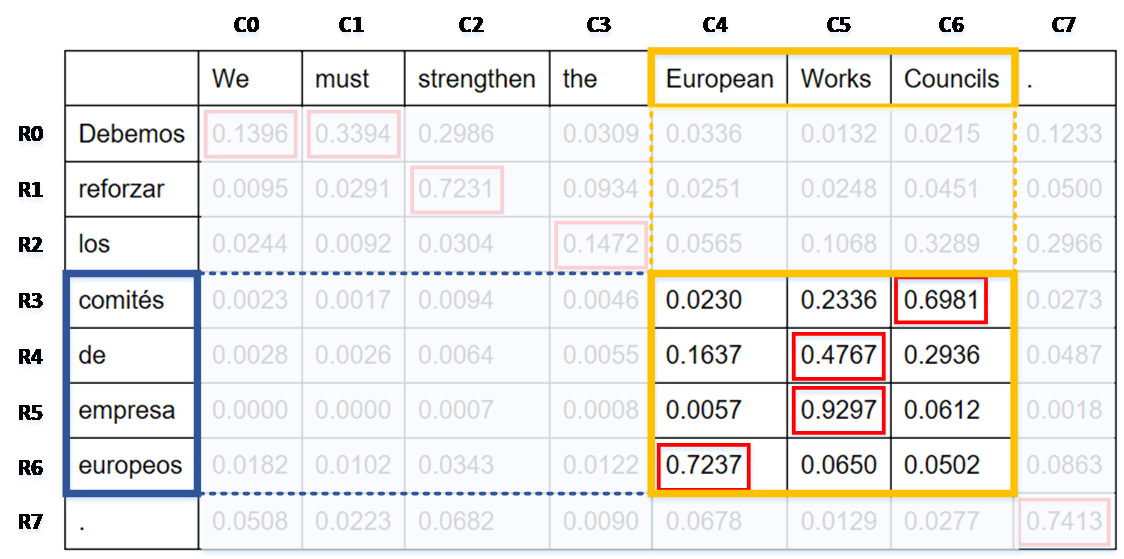
\includegraphics[scale=0.32]{Attn6.png}
	\caption{SE identification in a more complex sentence.}\label{Figure1}
\end{figure}

The significance level ($\alpha$) was set at 0.050 for all statistical tests. There was no significant relationship between $A$ and $B$, $X^2$ (2, $N$ = 6) = 0.86, $p$ = 0.649.

Figure~\ref{Figure2} provides an example of a normal distribution.

\begin{figure*}[htbp]
	\centering
	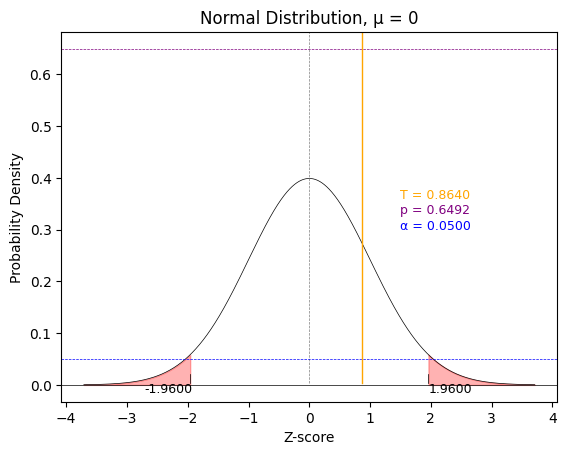
\includegraphics[scale=0.75]{Normal Distribution.png}
	\caption{Normal distribution.}\label{Figure2}
\end{figure*}

{\bf Captions}: Provide a caption for every illustration; number each one
sequentially in the form:  ``Figure 1: Caption of the Figure.'' ``Table 1:
Caption of the Table.''  Type the captions of the figures and 
tables below the body, using 11 point text.


\subsection{Equations}

Equations and mathematical expressions must be numbered so that they may be referenced. The following text provides examples of using equations, variables, and labels for numbering.
\begin{gather}
o = \sum_{t \in V}{\min (count(t,S_{1}), count(t, S_{2}))}\label{o}
\end{gather}

A credit value, $C$, is necessary to account for terminology tokens, $ t' $, that will not be counted when calculating the overlap, $o$, between the reference sentence, \textit{Refs}, and the modified prediction, \textit{P mod}, using orthographic matching.  Note that $C$ is only calculated on a translated sentence into which terminology has been injected.  If neither $S_{1}$ nor $S_{2}$ is the modified prediction, \textit{P mod}, there is no need to provide a credit for semantic equivalence and $ C $ will be zero.  Of necessity, the calculation of $ C $ assumes that all terminology injections are correct.
\begin{gather}
C=count(t', Pmod)\label{C}
\end{gather}

A Neural Machine Translation (NMT) system is a neural network that directly models
the conditional probability $ p(y|x) $ of translating a source
sentence, $ x_{1},...,x_{n} $, to a target sentence, $ y_{1},...,y_{m}$.		
\begin{gather}
    P_{C}=\lbrace{p_{0}, p_{1}, p_{2},\cdots, p_{r}}\rbrace\label{P} \\[-0.25em]
    M=\lbrace{P_{0}, P_{1}, P_{2},\cdots, P_{n}}\rbrace\label{M} \\[-0.25em]
    R_{S_{i}}=argmax(P_{C_{i}})\label{R}
\end{gather}

The entire attention matrix, then, can be expressed by Equation~\ref{M}, where \textit{n}
is the total number of columns in the matrix.

\subsection{Example References}

Like equations, linguistic examples must be numbered so they can be referenced. The following text demonstrates the use of examples, references, and labels for numbering.

A token cannot be removed from the vocabulary, but
it can be modified.  Doing so will allow replacement of a term.

For example, an NMT system might translate the source sentence given
in (\ref{ex1}) as the viable Spanish translation given in
(\ref{ex2}).\footnote{Sentences (1) and (2) are from EuroParl bitext.} However, in a given organizational context (\ref{ex3}) or
even (\ref{ex4}) might instead be the approved translation.

{\footnotesize
\ex[aboveexskip=1ex,belowexskip=0.5ex]
Your report is absolutely disgraceful.\label{ex1}
\xe
\ex[aboveexskip=0ex,belowexskip=0ex]
Su \underline{informe} es absolutamente vergonzoso.\label{ex2}
\xe
\ex[aboveexskip=0.5ex,belowexskip=1.5ex]
Su \underline{exposición} es absolutamente vergonzoso.\label{ex3}
\xe
\ex[aboveexskip=0.5ex,belowexskip=1.5ex]
Su \underline{exposición de alta calidad} es absolutamente vergonzoso.\label{ex4}
\xe
}





\section{Translation of non-English Terms}

It is also advised to supplement (that is, do not replace but provide in addition to) non-English characters and terms with appropriate transliterations and/or translations since not all readers understand all such characters and terms. Inline transliteration or translation can be represented in the order of: original-form transliteration ``translation''.

\section{Length of Submission}
\label{sec:length}

Submitted papers may consist of up to 8 pages of content plus up to two extra pages for references, but not less than 3 pages of content plus up to two extra pages for references.  Papers that do not conform to the specified length and formatting requirements may be
rejected without review and receive a failing grade.



\section*{Acknowledgments}

The acknowledgments section is optional and should go immediately before the references.  Do
not number the acknowledgments section.

% include your own bib file like this:
\bibliographystyle{bib_styles/acl_natbib_no_note}
\bibliography{bibliography}

\end{document}